\documentclass[11pt]{article}

\usepackage{classDM17}
\usepackage{mathtools}
\DeclarePairedDelimiter\ceil{\lceil}{\rceil}
\DeclarePairedDelimiter\floor{\lfloor}{\rfloor}

\title{Asmt 5: Regression}
\author{Gopal Menon\\Turn in through Canvas by 2:45pm: \\
Wednesday, April 12}
\date{}

\begin{document}
\maketitle


%
\section{Singular Value Decomposition (20 points)}
First we will compute the SVD of the matrix $A$ we have loaded
$$
[U,S,V] = svd(A)
$$
Then take the top $k$ components of $A$ for values of $k = 1$ through $k=10$ using

\begin{equation*}
\begin{aligned}
Uk &= U(:,1:k)\\
Sk &= S(1:k,1:k)\\
Vk &= V(:,1:k)\\
Ak &= Uk*Sk*Vk'\\
\end{aligned}
\end{equation*}

\paragraph{A: (10 points):} 
Compute and report the $L_2$ norm of the difference between $A$ and $Ak$ for each value of $k$ using
$$
norm(A-Ak,2)
$$

    \begin{table}[!h] 
    \centering
    \caption{$L_2$ norm of $A-Ak$ for each value of $k$}
    \label{AAkL2}
    \begin{tabular}{|c|c|}
      \hline
   $k$  & $L_2$ Norm  \\
      \hline      
      $1$ &      $40.483$  \\
      \hline
      $2$ &      $26.717$  \\
      \hline
      $3$ &      $25.000$  \\
      \hline
      $4$ &      $22.192$  \\
      \hline
      $5$ &      $17.675$  \\
      \hline
      $6$ &      $15.813$  \\
      \hline
      $7$ &      $13.351$  \\
      \hline
      $8$ &      $12.188$  \\
      \hline
      $9$ &      $9.1206$  \\
      \hline
      $10$ &      $9.0000$  \\
      \hline
    \end{tabular}
\end{table}

\paragraph{B (5 points):}
Find the smallest value $k$ so that the $L_2$ norm of $A-Ak$ is less than $10\%$ that of $A$; $k$ might or might not be larger than $10$.\\

The $L_2$ norm of $A$ is $120.19$ and $10\%$ of that is $12.019$. From table \ref{AAkL2}, we can see that the smallest value of $k$ such that the $L_2$ norm of $A-Ak$ is less than $10\%$ that of $A$ is $9$.

\paragraph{C (5 points):}

Treat the matrix as $1125$ points in $30$ dimensions. Plot the points in $2$ dimensions in the way that minimizes the sum of residuals squared.\\

The first two right singular vectors were used and all $1125$ points in $30$ dimensions were projected on them to get $1125$ points in $2$ dimensions. Since the first two singular vectors represent eigen vectors, this projection will result in the least sum of residuals squared. The plot is shown below in figure \ref{MinRes}.

\begin{figure}[!htb]
\centering
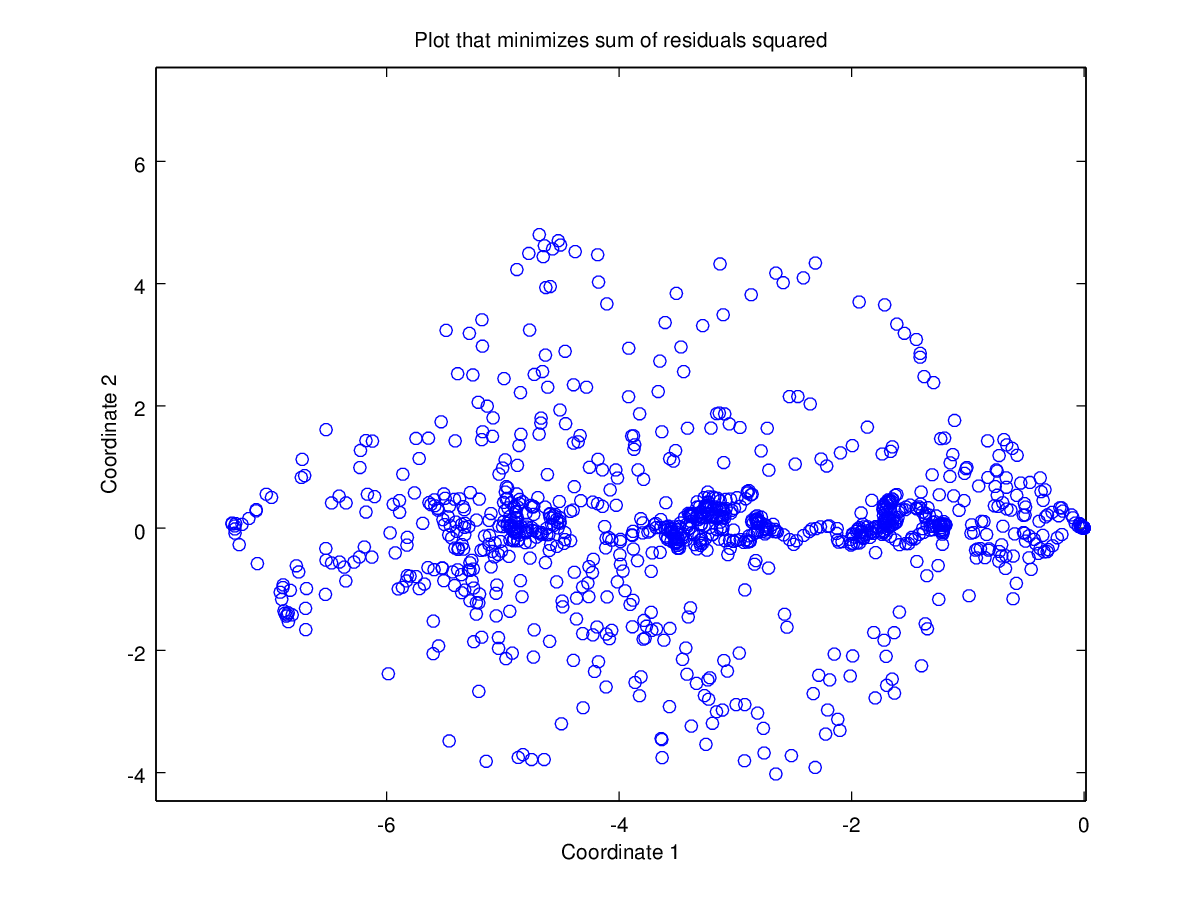
\includegraphics[width=5in]{figures/MinRes.png}
\caption{Points plotted in 2D to minimize sum of residuals squared}
\label{MinRes}
\end{figure} 

\section{Frequent Directions and Random Projections (40 points)}

\paragraph{A (20 points):}

\begin{itemize}
\item How large does $l$ need to be for the above error to be at most $\frac{\norm{A}_F^2}{10}$?\\
$$
\frac{\norm{A}_F^2}{10} = 1903.7
$$

\begin{table}[!h] 
    \centering
    \caption{Error for values of $l$}
    \label{ErrL}
    \begin{tabular}{|c|c|}
      \hline
   $l$  & Error  \\
      \hline      
      $3$ &      $2289.9$  \\
      \hline
      $4$ &      $1427.9$  \\
      \hline
      $5$ &      $965.01$  \\
      \hline
      $6$ &      $703.24$  \\
      \hline
      $7$ &      $494.53$  \\
      \hline
      $8$ &      $350.53$  \\
      \hline
      $9$ &      $247.37$  \\
      \hline
      $10$ &      $176.91$  \\
      \hline
    \end{tabular}
\end{table}

From table \ref{ErrL} we can see that with $l=4$, the error is at most $\frac{\norm{A}_F^2}{10}$.

\item How does this compare to the theoretical bound (e.g. for $k = 0$).

The theoretical bound is given by $\frac{\norm{A-A_k}_F^2}{l-k}$. When $k=0$, the bound becomes $\frac{\norm{A}_F^2}{l}$. This bound evaluates to $4759.3$ when $l=4$.

\item How large does $l$ need to be for the above error to be at most $\frac{\norm{A-A_k}_F^2}{10}$ for $k = 2$?

For $k = 2$, $\frac{\norm{A-A_k}_F^2}{10} = 295.18$. From table \ref{ErrL}, we can see that when $l=9$, the error is at most $\frac{\norm{A-A_k}_F^2}{10}$ for $k = 2$.

\end{itemize}

\paragraph{B (20 points):}

Estimate how large should l be in order to achieve $max_{\norm{x}=1} \left | \norm{Ax}^2 - \norm{Bx}^2 \right | \leq \frac{\norm{A}_F^2}{10}$. To estimate the relationship between $l$ and the error in this randomized algorithm, you will need to run multiple trials. Be sure to describe how you used these multiple trials, and discuss how many you ran and why you thought this was enough trials to run to get a good estimate.\\

In the random projections algorithm, we want a mapping $\mu : \mathbb{R}^d \rightarrow \mathbb{R}^l$ with $l \ll d$ where all $\mathbb{R}^d$ is compressed into $\mathbb{R}^l$. And we want all distances preserved so that for all points $a, a' \in A$
$$
(1-\varepsilon)\norm{a-a'} \leq \norm{\mu(a)-\mu(a')} \leq (1+\varepsilon)\norm{a-a'}
$$

The \textit{Johnson-Lindenstrauss Lemma} says that if the reduced number of dimensions $l=O\left ( \frac{1}{\varepsilon^2} \log \left (\frac{n}{\delta} \right ) \right )$, then for all $a, a' \in A$ the above bound is satisfied with a probability of at least $1-\delta$.\\

If $\varepsilon=0.10$ and $\delta=0.05$, then the number of rows we need to choose for the above bound to be satisfied with a probability of at least $0.95$ is

\begin{equation*}
\begin{aligned}\\
l&=O\left ( \frac{1}{\varepsilon^2} \log \left (\frac{n}{\delta} \right ) \right )\\
&= O\left ( \frac{1}{0.10^2} \log \left (\frac{1125}{0.05} \right ) \right )\\
&= O\left ( 100 \log \left (22500 \right ) \right )\\
&= O\left ( 435.22 \right )
\end{aligned}
\end{equation*}

\begin{table}[!h] 
    \centering
    \caption{Errors for number of rows $l$ in the random projection}
    \label{ErrRandProj}
    \begin{tabular}{|c|c|}
      \hline
   Number of rows $l$  & Error $=norm(A'*A - B'*B, 2)$ \\
      \hline      
      $430$ &      $1135.41$  \\
      \hline
      $431$ &      $1175.94$  \\
      \hline
      $432$ &      $1177.35$  \\
      \hline
      $433$ &      $1511.90$  \\
      \hline
      $434$ &      $610.41$  \\
      \hline
      $435$ &      $696.70$  \\
      \hline
      $436$ &      $1401.60$  \\
      \hline
      $437$ &      $1315.81$  \\
      \hline
      $438$ &      $287.31$  \\
      \hline
      $439$ &      $621.36$  \\
      \hline
      $440$ &      $435.97$  \\
      \hline
    \end{tabular}
\end{table}

The errors for various values of $l$ around $435$ are shown in table \ref{ErrRandProj}. In all the cases it is seen to be less than $\frac{\norm{A}_F^2}{10}$, which was already computed to be $1903.7$.

\section{Linear Regression (40 points)}

\paragraph{A (20 points):}
Solve for the coefficients $C$ (or $Cs$) using Least Squares and Ridge Regression with $s = {0.1, 0.3, 0.5, 1.0, 2.0}$ (i.e. s will take on one of those $5$ values each time you try, say obtaining $C05$ for $s = 0.5$). For each set of coefficients, report the error in the estimate $\hat{Y}$ of $Y$ as $norm(Y - X*C,2)$.

\begin{table}[!h] 
    \centering
    \caption{Least Squares Regression Error}
    \label{ErrOls}
    \begin{tabular}{|c|}
      \hline
    Error \\
      \hline      
      $25.823822$  \\
      \hline
    \end{tabular}
\end{table}
\begin{table}[!h] 
    \centering
    \caption{Ridge Regression Error}
    \label{ErrRidge}
    \begin{tabular}{|c|c|}
      \hline
   $s$  & Error \\
      \hline      
      $0.1$ &      $25.823824$  \\
      \hline
      $0.3$ &      $25.823943$  \\
      \hline
      $0.5$ &      $25.824676$  \\
      \hline
      $1.0$ &      $25.833907$  \\
      \hline
      $2.0$ &      $25.919640$  \\
      \hline
    \end{tabular}
\end{table}

\paragraph{B (20 points):}

Create three row-subsets of $X$ and $Y$

\begin{itemize}
\item $X1 = X(1:66,:)$ and $Y1 = Y(1:66)$
\item $X2 = X(34:100,:)$ and $Y2 = Y(34:100)$
\item $X3 = [X(1:33,:); X(67:100,:)]$ and $Y3 = [Y(1:33); Y(67:100)]$
\end{itemize}

Repeat the above procedure on these subsets and \textit{cross-validate} the solution on the remainder of $X$ and $Y$. Specifically, learn the coefficients $C$ using, say, $X1$ and $Y1$ and then measure $norm(Y(67:100) - X(67:100,:)*C,2)$.

\begin{table}[!h] 
    \centering
    \caption{Least Squares Regression Error}
    \label{ErrOls2}
    \begin{tabular}{|c|c|}
      \hline
   Training Subsets  & Error \\
      \hline      
      $X1, Y1$ &      $14.787131$  \\
      \hline
      $X2, Y2$ &      $14.525954$  \\
      \hline
      $X3, Y3$ &      $23.194199$  \\
      \hline
      Average &      $17.502428$  \\
      \hline
    \end{tabular}
\end{table}

\begin{table}[!h] 
    \centering
    \caption{Ridge Regression Error}
    \label{ErrRidge2}
    \begin{tabular}{|c|c|c|c|c|c|}
      \hline
   Training Subsets  & $Error_{s=0.1}$ & $Error_{s=0.3}$ &$Error_{s=0.5}$ &$Error_{s=1.0}$ &$Error_{s=2.0}$  \\
      \hline      
      $X1, Y1$ &      $14.785569$  & $14.773048$ & $14.747842$ & $14.627345$ & $14.167225$ \\
      \hline
      $X2, Y2$ &      $14.525810$   & $14.525195$ & $14.526353$ & $14.555734$ & $14.809322$ \\
      \hline
      $X3, Y3$ &      $23.195206$   & $23.203230$ & $23.219111$ & $23.292336$ & $23.610916$ \\
      \hline
      Average &      $17.502195$   & $17.500491$ & $17.497769$ & $17.491805$ & $17.529154$ \\
      \hline
    \end{tabular}
\end{table}

Which approach works best (averaging the results from the three subsets): Least Squares, or for which value of $s$ using Ridge Regression?\\

The approach that worked best was for Ridge Regression with $s=1.0$, which had the lowest average error.

\end{document}
